\documentclass[crop=false]{standalone}
\usepackage{geometry}
\usepackage{amsmath}
\usepackage{amssymb}
\usepackage[dvips]{graphicx}
\usepackage{psfragx}
\usepackage{pst-all}
\usepackage{cmbright}

% Set the size of the final .pdf based on the figure size
% The 'standalone' class must be loaded with the 'crop=false' option,
% and together with the geometry package. Otherwise the final figure
% will be slightly larger than the original size.
\setlength{\parindent}{0cm}
\def\figure{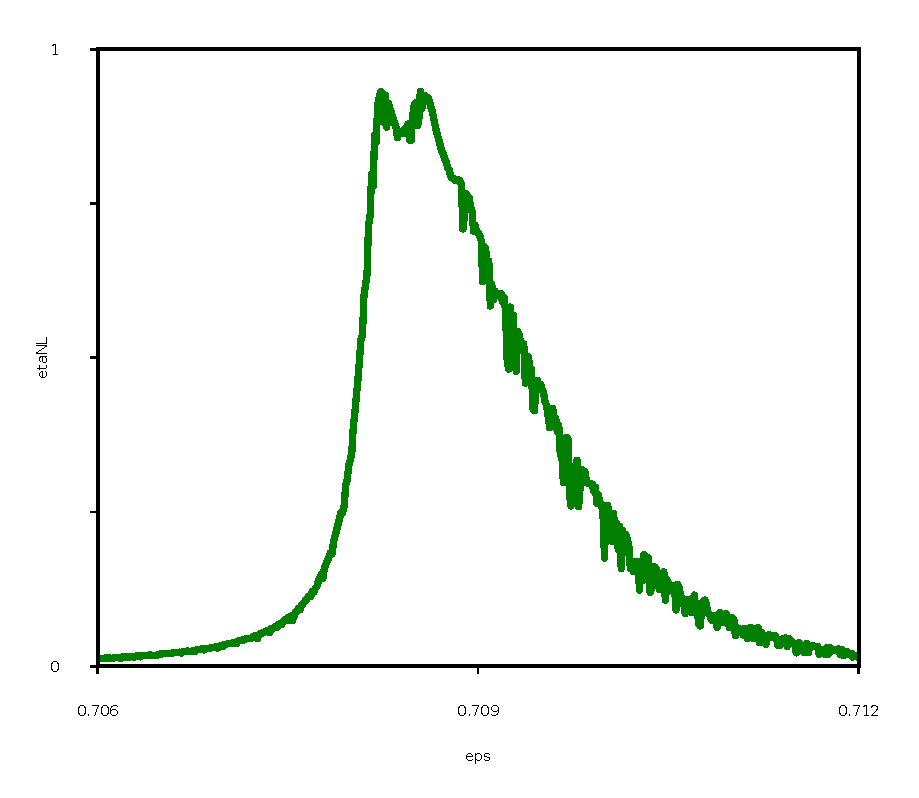
\includegraphics{Fig3.eps}}
\newlength\figurewidth
\newlength\figureheight
\settoheight\figureheight{\figure}
\settowidth\figurewidth{\figure}
\geometry{paperwidth=\figurewidth,paperheight=\figureheight,margin=0in}

\begin{document}
		\fontsize{24}{28.8} \selectfont
        \psfrag{pAp}[c][c]{(a)}
        \psfrag{pBp}[c][c]{(b)}
        \psfrag{pCp}[c][c]{(c)}
		\psfrag{-2}[B][B]{\hspace{-1ex}$-2$}
		\psfrag{0}[B][B]{$0$}
		\psfrag{0.5}[B][B]{$0.5$}
		\psfrag{1}[B][B]{$1$}
		\psfrag{2}[B][B]{$2$}
        \psfrag{2.2}[B][B]{$2.2$}
        \psfrag{2.4}[B][B]{$2.4$}
        \psfrag{2.6}[B][B]{$2.6$}
		\psfrag{3}[B][B]{$3$}
		\psfrag{6}[B][B]{$6$}
		\psfrag{9}[B][B]{$9$}
        \psfrag{-4}[B][B]{\hspace{-1ex}$-4$}
		\psfrag{4}[B][B]{$4$}
		\psfrag{5}[B][B]{$5$}
		\psfrag{10}[B][B]{$10$}
		\psfrag{8}[B][B]{$8$}
		\psfrag{12}[B][B]{\hspace{1ex}$12$}
		\psfrag{0.0}[B][B]{$0.0$}
		\psfrag{1.2}[B][B]{\scriptsize$1.2$}
		\psfrag{0.8}[B][B]{\scriptsize$0.8$}
		\psfrag{1.0}[B][B]{\scriptsize$1.0$}
        \psfrag{0.706}[B][B]{\hspace{2ex}$0.706$}
		\psfrag{0.706ins}[B][B]{\scriptsize$0.706$}
		\psfrag{0.709}[B][B]{$0.709$}
        \psfrag{0.712ins}[B][B]{\hspace{-2.4ex}\scriptsize$0.712$}
        \psfrag{0.712}[B][B]{\hspace{-3.9ex}$0.712$}
        \psfrag{nav/nB}[B][B]{\hspace{-1.8ex}\scriptsize$\frac{\bar{n}_\alpha}{n^\mathrm{th}_\alpha}$}
        \psfrag{g=0.05GS}[B][B]{$\lambda\!=\!0.05\Gamma_S$}
        \psfrag{g=0.2GS}[B][B]{$\lambda\!=\!0.2\Gamma_S$}
        \psfrag{nL}[B][B]{\scriptsize$\bar{n}_L$}
        \psfrag{nR}[B][B]{\scriptsize$\bar{n}_R$}
        \psfrag{eps}[B][B]{$\epsilon\ [\Gamma_S]$}
        \psfrag{eps2}[B][B]{\scriptsize$\epsilon\ [\Gamma_S]$}
        \psfrag{eV}[B][B]{$eV\ [\Gamma_S]$}
        \psfrag{etaL}[B][B]{$\eta^{(L)}_{\mathrm{loc}}$}
        \psfrag{etaNL}[B][B]{$\eta_{\mathrm{NL}}$}
		\psfrag{IR}[B][b]{$I_\alpha$ [$e\Gamma$]}
        \psfrag{d=wL-wR}{\scriptsize$\bar{\delta}\!\!=\!\!\omega_L\!\!-\!\omega_R$}
        \psfrag{d=wR}{\scriptsize$\bar{\delta}\!\!=\!\!\omega_R$}
        \psfrag{d=wL}{\scriptsize$\bar{\delta}\!\!=\!\!\omega_L$}
        \psfrag{d=2wR}{\scriptsize$\bar{\delta}\!\!=\!\!2\omega_R$}

        \figure
\end{document}
